\section{Experimentación}

	\subsection{\emph{PageRank} y páginas web}

	A continuación, se presentan los experimentos que se realizaron. Con el código del trabajo práctico se incluye una serie de scripts de \emph{bash} que permiten recrear los experimentos realizados, como así también los gráficos que se incluyen en este informe; esto puede hacerse ingresando al directorio \texttt{exp} dentro de la raíz, y ejecutando el comando \texttt{./exp{i}.sh}, siendo \texttt{i} el número de experimento.

		\subsubsection{Experimento 1}
			\subsubsection*{Presentación}
			En el primer experimento se quiere observar como varía el tiempo de ejecución a medida que se modifica el valor del parámetro $c$, para lograr que la norma Manhattan entre dos iteraciones consecutivas sea menor que la tolerancia indicada. Para ello se toma una determinada cantidad de páginas web que no se modificarán a lo largo del experimento y se ejecutará el programa para diferentes valores de $c$. Con el fin de mejorar la precisión de los resultados y evitar posibles interferencias (por ejemplo, las generadas por otras tareas que pueda estar ejecutando la computadora) cada medición se repitió 10 veces, tomando luego el promedio de los datos obtenidos

			\subsubsection*{Hipótesis}
			Se conjetura que cuanta mayor sea la probabilidad de teletransportarse de una página a otra, menos tiempo va a tardar el algoritmo en llegar al estado en el que la tolerancia sea menor que la norma Manhattan. $(1-c)$ indica cuál es la probabilidad de, estando en cualquier página, teletransportarse a otra. Por esto es que cuanto más chico sea el valor de $c$, menos tiempo de ejecución demorará el algoritmo.

			\subsubsection*{Datos de entrada} 
			Se toman 13 páginas con 16 \emph{links}. Además el parámetro $c$ toma los valores \texttt{0, 0.1, 0.2, 0.3, 0.4, 0.5, 0.6, 0.7, 0.8, 0.9, 1}. La tolerancia es de \texttt{0.00001}. Se eligió la cantidad de páginas y el valor de la tolerancia arbitrariamente, procurando que los casos de prueba no fueran excesivamente grandes para no prolongar innecesariamente la duración de las pruebas. 

			\subsubsection*{Resultados}
				{\centering \begin{tabular}{c}
			      % 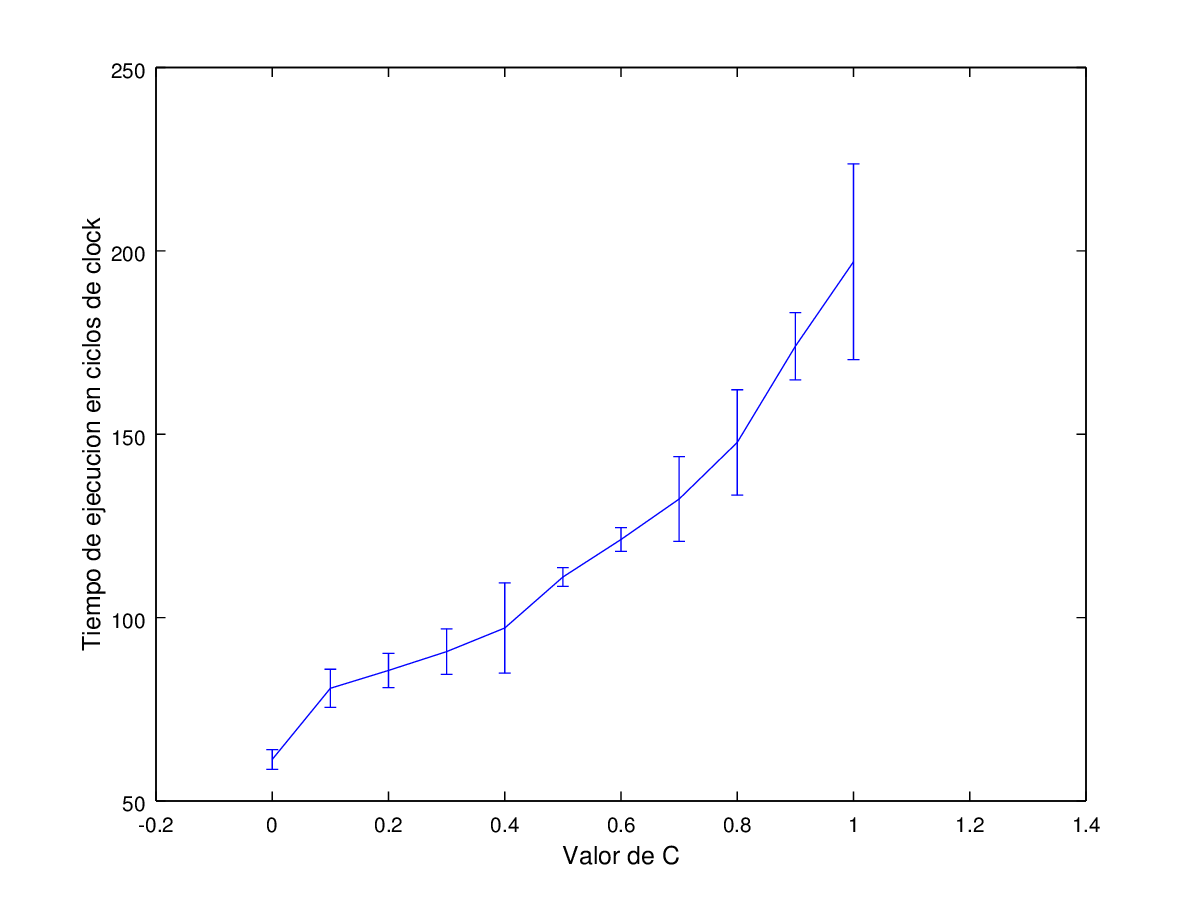
\includegraphics[width=12cm]{../../src/exp/graficos/exp1.png} \\
			    \end{tabular}}

			\subsubsection*{Discusión} 
			Como se puede observar en el experimento, a medida que aumenta el valor de c, aumenta el tiempo de ejecución. Esto se debe a que la matriz inicial no es homogénea y la que formamos a partir del c si lo es. Así, cuando la segunda toma dicha importancia, el sistema tiende más rápido a ser homogéneo y requiere menos iteraciones del ciclo para lograr una norma menor a la tolerancia deseada. 


		\subsubsection{Experimento 2}
			\subsubsection*{Presentación}
			Con este experimento se pretende observar la diferencia en el tiempo de ejecución cuando se varía la cantidad de \emph{links} en una determinada cantidad de páginas, manteniendo el valor de la tolerancia constante.
			Para ello se utilizan listas de páginas diferentes como parámetro de entrada en cada una de las ejecuciones a comparar, pero manteniendo la cantidad de las mismas. Se toma el tiempo que se demora en ejecutar el algoritmo y se lo divide por la cantidad de iteraciones realizadas. Esto permite obtener un promedio del tiempo que demora por cada una de las iteraciones del ciclo.
		
			\subsubsection*{Hipótesis} 
			Suponemos que variar la cantidad de \emph{links} altera más el tiempo de ejecución que variar la cantidad de páginas sin que estén relacionadas entre ellas. Esto se debe a que, dada la forma en la que está implementado el algoritmo, sacando provecho del hecho de que la matriz es esparsa, agregar entradas a la matriz de adyacencia tendrá un mayor impacto sobre la cantidad de operaciones a realizar. Por lo tanto, se espera observar que el tiempo de ejecución aumente a medida que la cantidad de relaciones entre páginas sea mayor.

			\subsubsection*{Datos de entrada} 		
			Para este experimento se toman 50 páginas. La cantidad de \emph{links} entre ellas varía, tomando los valores \texttt{4, 32, 70, 105, 130, 160}. Estos valores fueron elegidos a modo de análisis. Para generarlos se creó una red a partir de diferentes páginas web interconectadas entre sí. Luego se borraron algunas páginas, eliminando una determinada cantidad de \emph{links}, y se agregaron nuevas páginas desconectadas totalmente de las ya existentes. De esta forma, no se disminuyó la cantidad de páginas pero sí la de \emph{links}. Además el valor de $c$ es \texttt{0.85} y el valor de la tolerancia es \texttt{0.00001}. El valor de $c$ y de la tolerancia fueron elegidos arbitrariamente, procurando que los casos de prueba no fueran excesivamente grandes para no prolongar innecesariamente la duración de las pruebas. 
			
			\subsubsection*{Resultados}
				{\centering \begin{tabular}{c}
			      % 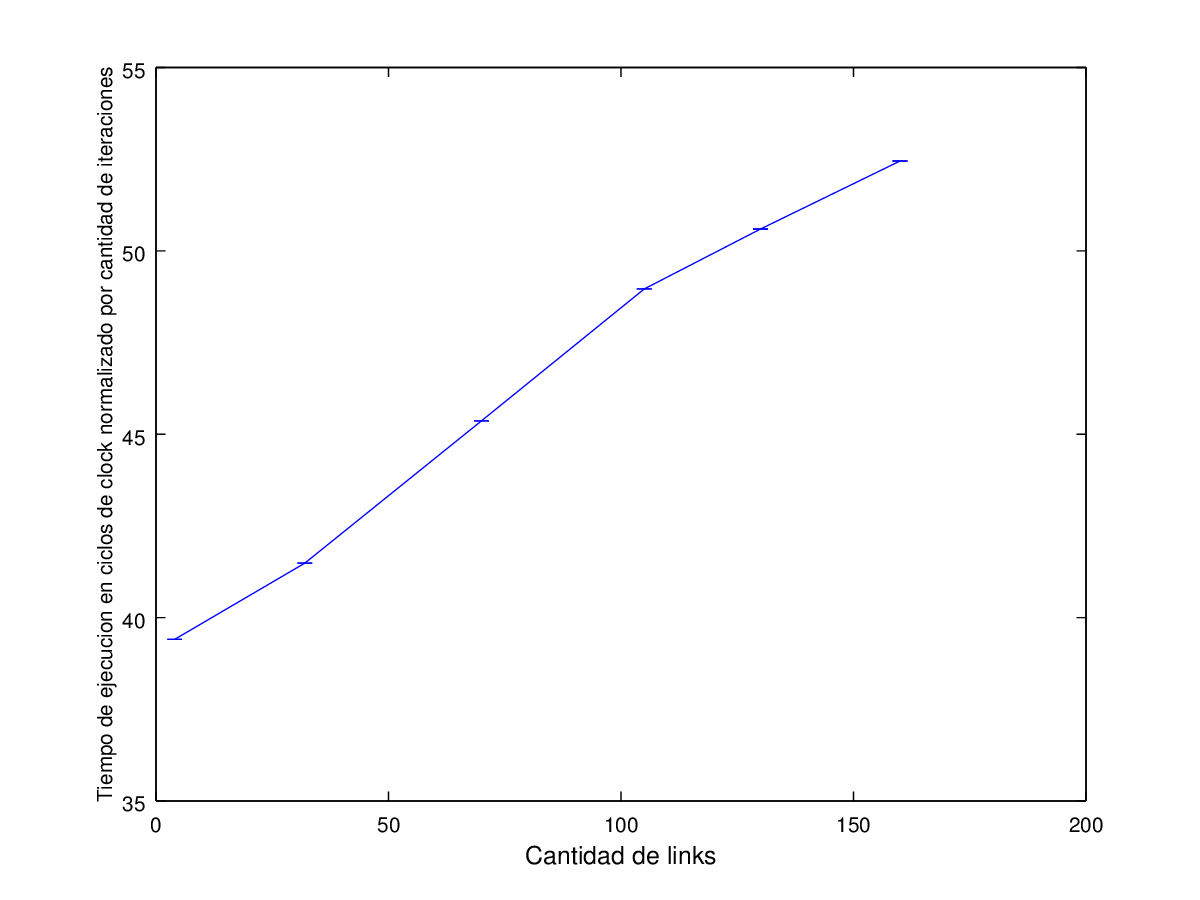
\includegraphics[width=12cm]{../../src/exp/graficos/exp2.png} \\
			    \end{tabular}}


			\subsubsection*{Discusión}
			Como se puede observar en el gráfico, a medida que aumentan las relaciones entre las páginas el tiempo de ejecución es mayor.  

		\subsubsection{Experimento 3}
			\subsubsection*{Presentación}
			En este experimento también se observa la diferencia en el tiempo de ejecución, pero comparando igual cantidad de páginas y relaciones entre las mismas y variando el valor de la tolerancia.
			Para ello se toma como parámetro de entrada en cada una de las ejecuciones una misma lista de páginas y se incrementa el valor de la tolerancia.

			\subsubsection*{Hipótesis} 
			Creemos que cuanto mayor sea la tolerancia, menor será el tiempo de ejecución del algoritmo. Esto se debe a que el algoritmo termina cuando la diferencia Manhattan es menor que la tolerancia. Entonces cuanto más grande sea el valor de la tolerancia, más rápido se cumplirá la condición para salir del ciclo y menos tardará en ejecutarse el algoritmo. Suponemos que para los valore mas chicos de tolerancia el tiempo de ejecución será altamente mayor que para valores de tolerancia cercanos a 1. Es decir, el crecimiento será exponenecial a medida que disminuimos el valor de la tolerancia.

			\subsubsection*{Datos de entrada} 
			Se toman 13 páginas con 16 \emph{links}. Además la tolerancia toma los siguientes valores: \texttt{0.000001, 0.000005, 0.00001, 0.00005, 0.0001, 0.0005, 0.001, 0.005, 0.01, 0.1, 0.3, 0.5, 0.7}. El parámetro $c$ es igual a \texttt{0.85}. El valor de $c$ y la cantidad de páginas fueron elegidos arbitrariamente, procurando que los casos de prueba no fueran excesivamente grandes para no prolongar innecesariamente la duración de las pruebas. Los valores de la tolerancia fueron tomados a modo de análisis teniendo en cuenta que el objetivo del experimento. 

			\subsubsection*{Resultados}
				{\centering \begin{tabular}{c}
			      % 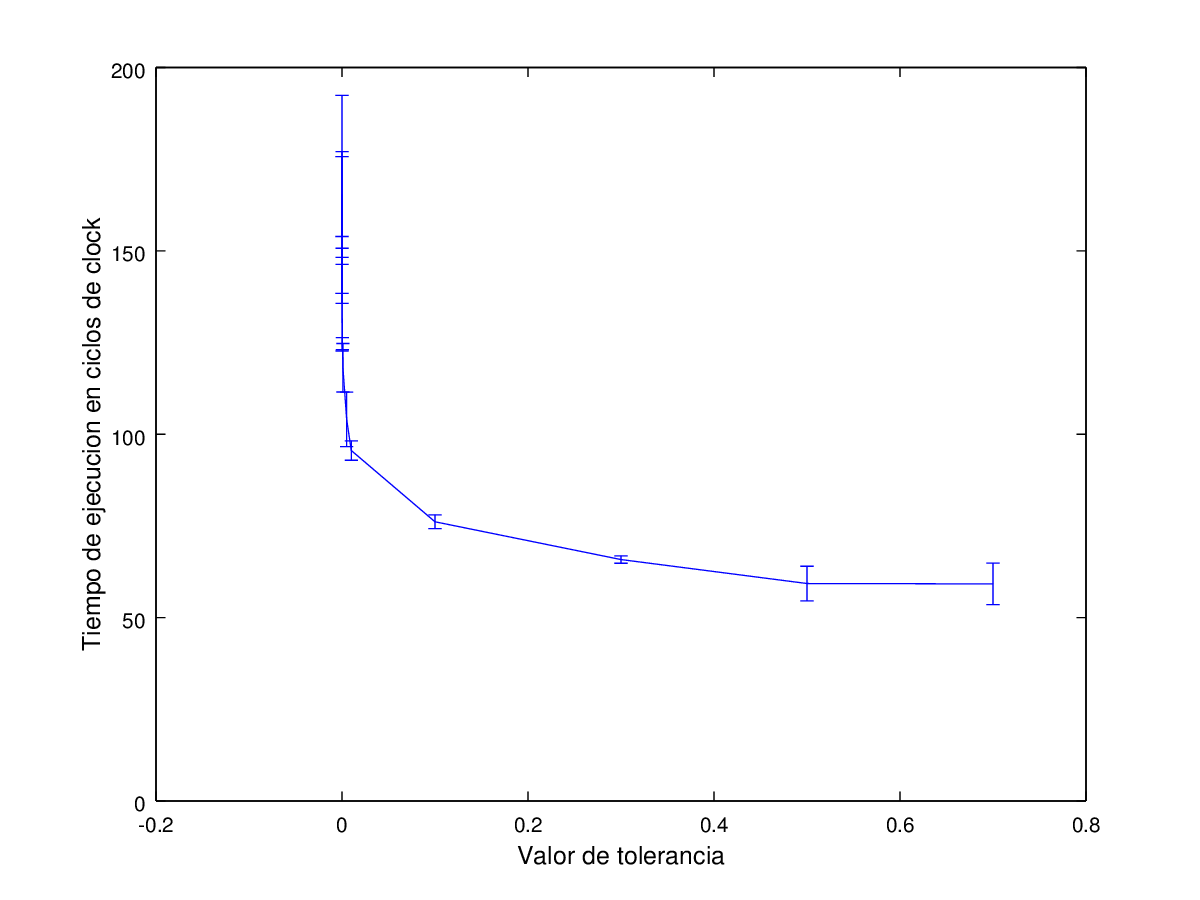
\includegraphics[width=12cm]{../../src/exp/graficos/exp3.png} \\
			    \end{tabular}}

			\subsubsection*{Discusión}
			Como se puede ver en el gráfico, al aumentar la tolerancia disminuye el tiempo de ejecución linealmente. Al estar en escala logaritmica, esto quiere decir que la función decrece de forma exponencial. Para valores de tolerancia cercanos a 1, la cantidad de iteraciones a realizar es notoriamente menor que para valores de tolerancia cercanos a 0. Esto sucede ya que el método converge cada vez mas lento, entonces cuando la tolerancia toma valores muy chicos las ultimas iteraciones modifican muy poco el vector por lo que se requieren más iteraciones para acercarse al resultado.
			Además se puede observar que hasta el valor de tolerancia 0.01 la variación en tiempo de ejecución dependiendo del valor de la tolerancia es mínimo. Cuando ese valor es menor que 0.01 el tiempo de ejecución se incrementa notoriamente. Dejamos a experimentos futuros ver cuál es el valor en el que el tiempo de ejecución es muy grande. En este sentido, se pudo confirmar la hipótesis.   

	\subsubsection{Experimento 4}
		\subsubsection*{Presentación}
		Otra de las pruebas consiste en comparar los \emph{rankings} formados al ejecutar los algoritmos de \emph{PageRank} y el de \textsc{In-deg}. Primero se analiza una lista de páginas de entrada en la que una de ellas sea apuntada por el resto (Web 1). 

		Luego se realiza la comparación con una lista en la que hayan dos páginas (a las que llamaremos página 1 y página 3) que sean apuntadas por varias paginas. Además, la página 3 tendrá un link a la 1. También se cuenta con otra (a la que llamaremos página 2) que apunta y es apuntada por la página 1, tal como se muestra en el siguiente esquema (Web 2):

			\begin{figure}[h]

				\begin{center}
					\begin{tabular}{@{\extracolsep{2cm}} cc}
				      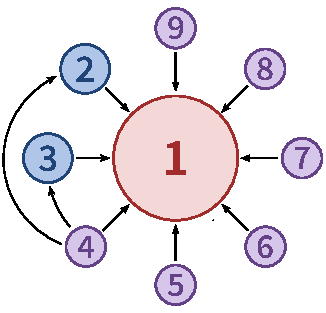
\includegraphics{imagenes/exp4-graph1.pdf} & 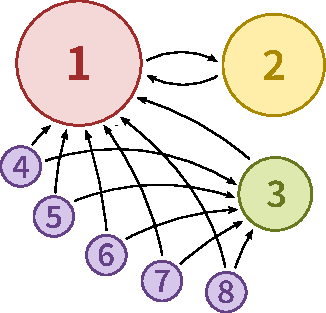
\includegraphics{imagenes/exp4-graph2.pdf} \\
				      {\small \strong{Web 1}} & {\small \strong{Web 2}}
				    \end{tabular}
			    \end{center}

		    	\caption{Redes utilizadas como datos de entrada para el Experimento 4} \label{fig:exp4-webs}

		    \end{figure}

			\subsubsection*{Hipótesis} 
			En el primero, suponemos que los \emph{rankings} obtenidos en ambos casos serán iguales ya que existe una sola página principal y el resto tiene igual cantidad de relaciones. Por otro lado, en el segundo notaremos diferencias. Llamaremos enlace fuerte a aquel que va de una página que es apuntada por muchas otras hacia otra página. El método \emph{PageRank} tiene en cuenta cuál es el peso de los \emph{links} que apuntan a las distintas páginas. En el caso de \textsc{In-deg}, solo se utiliza como información la cantidad de enlaces que llegan a cada una de las distintas páginas.

			En el experimento, si consideramos el método \emph{PageRank}, la página 1 quedará en primer lugar, ya que es la que recibe más \emph{links} a la misma, pero en segundo lugar quedará la página 2. Esto se debe a que el enlace de la 1 a la 2 es un enlace muy fuerte. En el caso de \textsc{In-deg}, esto no sucede ya que este método solo toma en cuenta que existe un único link hacia la página 2. Por lo tanto en \emph{PageRank} las posiciones serán 1-2-3 y luego el resto. En \textsc{In-deg} tendremos primero a la página 1 seguida de la 3, luego la 2 y finalmente el resto.

			\subsubsection*{Datos de entrada}
			Para la Web 1, se tomaron 9 páginas con 10 \emph{links}. Para la Web 2, se tomaron 8 páginas con 13 \emph{links}.  

			El valor de $c$ es \texttt{0.85} y el valor de tolerancia es \texttt{0.00001}. 
			 		
			\subsubsection*{Resultados}

			   \begin{center}
	      			\begin{tabular}{c|c|c} 
			      		\hline
			  				\multicolumn{3}{c}{\emph{Ranking} Web 1 - \emph{PageRank}} \\
			 			\hline
	        			Posición & Nodo & Puntaje \\ \hline
	         			1 & 1 & 0.473848 \\
	        			2 & 8 & 0.078821 \\
	        			3 & 9 & 0.078821 \\
	        			4 & 2 & 0.061418 \\
	        			5 & 3 & 0.061418 \\
	        			6 & 4 & 0.061418 \\
	        			7 & 5 & 0.061418 \\
	        			8 & 6 & 0.061418 \\
	        			9 & 7 & 0.061418 
	      			\end{tabular} 

	      			\begin{tabular}{c|c|c}
			      		\hline
			  				\multicolumn{3}{c}{\emph{Ranking} Web 1 - \textsc{In-deg}} \\
			 			\hline
	        			Posición & Nodo & Puntaje \\ \hline
	         			1 & 1 & 0.8 \\
	        			2 & 8 & 0.1 \\
	        			3 & 9 & 0.1 \\
	        			4 & 2 & 0 \\
	        			5 & 3 & 0 \\
	        			6 & 4 & 0 \\
	        			7 & 5 & 0 \\
	        			8 & 6 & 0 \\
	        			9 & 7 & 0 
	      			\end{tabular}

	      			\begin{tabular}{c|c|c}
			      		\hline
			  				\multicolumn{3}{c}{\emph{Ranking} Web 2 - \emph{PageRank}} \\
			 			\hline
	        			Posición & Nodo & Puntaje \\ \hline
	         			1 & 1 & 0.448059 \\
	        			2 & 2 & 0.448059 \\
	        			3 & 3 & 0.058594 \\
	        			4 & 4 & 0.058594 \\
	        			5 & 5 & 0.018750 \\
	        			6 & 6 & 0.018750 \\
	        			7 & 7 & 0.018750 \\
	        			8 & 8 & 0.018750
	      			\end{tabular}
	    		
	      			\begin{tabular}{c|c|c}
			      		\hline
			  				\multicolumn{3}{c}{\emph{Ranking} Web 2 - \textsc{In-deg}} \\
			 			\hline
	        			Posición & Nodo & Puntaje \\ \hline
	         			1 & 1 & 0.538462 \\
	        			2 & 3 & 0.384615 \\
	        			3 & 2 & 0.076923 \\
	        			4 & 4 & 0 \\
	        			5 & 5 & 0 \\
	        			6 & 6 & 0 \\
	        			7 & 7 & 0 \\
	        			8 & 8 & 0 \\
	      			\end{tabular}
	    	\end{center}

			\subsubsection*{Discusión} 
			Como podemos ver en los \emph{rankings} del primer análisis en ambos casos quedan iguales. En cambio, en el segundo observamos variaciones, ya que en la lista de entrada el peso de todos los enlaces no es el mismo, es decir, hay enlaces más fuertes que otros. A diferencia de \emph{PageRank}, el método \textsc{In-deg} no tiene en cuenta esta propiedad. Por lo tanto, si en las páginas de entrada todos los \emph{links} tienen igual fuerza, el resultado obtenido por ambos métodos no difiere. 


	\subsection{\emph{GeM} y ligas deportivas}
		
		\subsubsection{Experimento 1}
		\subsubsection*{Presentación}
		En este experimento se verá la diferencia entre los métodos de \emph{GeM} y el de la \acr{AFA} para determinar el \emph{ranking} de una liga deportiva. Para ello se tomará como parámetro de entrada una tabla con los partidos, sus respectivas fechas, y sus resultados. En la misma, deberá existir un equipo que ocupe una de las primaras posiciones en la tabla de \emph{rankings} que haya perdido contra otro que ocupa una de las últimas. Observaremos la diferencia entre el \emph{ranking} generado por cada uno de los métodos.

			\subsubsection*{Hipótesis} 
			Cuando se juega un partido entre dos equipos, en el método de \emph{GeM} se tendrá en cuanta que tan fuerte son los equipos involucrados y cual fue la diferencia de goles en el partido. En cambio, en el método de la \acr{AFA} el ganador recibirá 3 puntos sin importar los resultados ni las posiciones que los mismos tenían hasta el momento. Esto puede generar diferencias en el \emph{ranking} ya que cada método considera distinta información para determinar las nuevas posiciones. 
			
			Por otro lado, si un equipo que se encuentra en las últimas posiciones de la tabla juega contra uno que esta en las primeras y gana el peor, para el método de la \acr{AFA} es exactamente igual que haya jugado con cualquier otro. Para \emph{GeM}, al tener en cuenta que tan fuertes son los equipos, esto generará que el nuevo vencedor quede en una mejor posición en la tabla. Así en este método entre dos fechas se pueden generar saltos, es decir, un equipo puede pasar de tener una muy mala posición en la tabla a estar dentro de los mejores solo por haber ganado un partido contra un equipo fuerte. En el método de la \acr{AFA} no pasa ya que sólo se le sumarán 3 puntos al equipo triunfador.		

			\subsubsection*{Datos de entrada} 
				Resultados del Torneo de Primera División del Fútbol Argentino hasta la Fecha 23. El valor de $c$ es \texttt{0.85} y el valor de tolerancia es \texttt{0.00001}. Se eligió el valor de c y el de la tolerancia arbitrariamente, procurando que los casos de prueba no fueran excesivamente grandes para no prolongar innecesariamente la duración de las pruebas. 
. 

			\subsubsection*{Resultados}

				\begin{center}
	      			\begin{tabular}{|c|c|c|} 
			      		\hline
			  				\multicolumn{3}{c}{\emph{Ranking} Liga Deportiva - \emph{GeM}} \\
			 			\hline
	        			Posición & Equipo & Puntaje \\ \hline
	         			1 & Boca Juniors & 0.080913 \\
	        			2 & Aldosivi & 0.069879 \\
	        			3 & River Plate & 0.069065 \\
	        			4 & San Lorenzo & 0.058309 \\
	        			5 & San Martín (SJ) & 0.051788 \\
	        			6 & Racing Club & 0.051674 \\
	        			7 & Rosario Central & 0.046326 \\
	        			8 & Quilmes & 0.045206 \\
	        			9 & Newell's Old Boys & 0.043581 \\
	        			10 & Vélez Sarsfield & 0.039828 \\
	        			11 & Gimnasia y Esgrima (LP) & 0.035738 \\
	        			12 & Estudiantes (LP) & 0.034629 \\
	        			13 & Belgrano & 0.033908 \\
	        			14 & Banfield & 0.032996 \\
	        			15 & Unión & 0.028015 \\
	        			16 & Defensa y Justicia & 0.027041 \\
	        			17 & Lanús & 0.026036 \\
	   					18 & Independiente & 0.023666 \\
	   					19 & Tigre & 0.023078 \\
	   					20 & Sarmiento & 0.022266 \\
	   					21 & Olimpo & 0.021956 \\
	   					22 & Crucero del Norte & 0.021713 \\
	  					23 & Arsenal & 0.018678 \\
	   					24 & Argentinos Juniors & 0.017951 \\
	   					25 & Tempreley & 0.017670 \\
	   					26 & Huracán & 0.013740 \\
	   					27 & Godoy Cruz & 0.013541 \\
	   					28 & Atlético de Rafaela & 0.011738 \\
	   					29 & Colón & 0.011141 \\
	   					30 & Nueva Chicago & 0.007928 

	      			\end{tabular} 
	      			    \begin{tabular}{|c|c|c|} 
			      		\hline
			  				\multicolumn{3}{c}{\emph{Ranking} Liga Deportiva - \acr{AFA}} \\
			 			\hline
	        			Posición & Equipo & Puntaje \\ \hline
						    1 & San Lorenzo & 0.054289 \\
						    2 & Boca Juniors & 0.053203 \\
						    3 & Racing Club & 0.049946 \\
						    4 & Rosario Central & 0.048860 \\
						    5 & River Plate & 0.047774 \\
						    6 & Independiente & 0.041260 \\
						    7 & Belgrano & 0.041260 \\
						    8 & Estudiantes (LP) & 0.041260 \\
						    9 & Tigre & 0.040174 \\
						   10 & Banfield & 0.040174 \\
						   11 & Lanús & 0.039088 \\
						   12 & Gimnasia y Esgrima (LP) & 0.038002 \\
						   13 & Quilmes & 0.034745 \\
						   14 & San Martín (SJ) & 0.034745 \\
						   15 & Unión & 0.033659 \\
						   16 & Tempreley & 0.030402 \\
						   17 & Argentinos Juniors & 0.028230 \\
						   18 & Newell's Old Boys & 0.028230 \\
						   19 & Aldosivi & 0.028230 \\
						   20 & Vélez Sarsfield & 0.027144 \\
						   21 & Defensa y Justicia & 0.026059 \\
						   22 & Sarmiento & 0.026059 \\
						   23 & Olimpo & 0.024973 \\
						   24 & Colón & 0.024973 \\
						   25 & Godoy Cruz & 0.023887 \\
						   26 & Huracán & 0.022801 \\
						   27 & Atlético de Rafaela & 0.021716 \\
						   28 & Arsenal & 0.018458 \\
						   29 & Nueva Chicago & 0.015201 \\
						   30 & Crucero del Norte & 0.015201 \\

	      			\end{tabular} 
	      	\end{center}

			\subsubsection*{Discusión}

			Como podemos ver en las tablas de \emph{rankings}, los ordenes no son exactamente iguales. Por ejemplo, mirando el equipo 1 (Aldosivi), en el \emph{ranking} de la \acr{AFA} se encuentra en la posición 20 y cuando usamos el método de \emph{GeM} éste esta en la posición 2. Esto se debe a que Aldosivi le ganó tanto al equipo 24 (San Lorenzo) como al 7 (Boca Juniors), que se encontraban primero y segundo en la tabla de posiciones de la \acr{AFA}, respectivamente. Por esto, en \emph{GeM} sube muchas posiciones mientras que con la \acr{AFA} solo se le otorgan 3 puntos por cada uno de los dos partidos.

